\documentclass{beamer}

\usepackage{beamerthemesplit}
\usepackage[utf8]{inputenc}
\usecolortheme{rose}
\usepackage{slovak}
\usepackage{subfigure}

\def\languagename{english}
\def\dd{\;{\rm d}\,}
\def\imag{\hat{\imath}}

\def\mytitle{Fourierova transformácia a jej použitie}
\def\myauthor{Peter Perešíni}
\date{\today}
\setbeamercovered{transparent}

\title\mytitle
\author\myauthor

%%% {{{ Section autonumbering
%\AtBeginSection[]
%{
%  \frame<handout:0>
%  {
%    \frametitle{Prehľad}
%    \tableofcontents[currentsection,hideallsubsections]
%  }
%}
%
%\AtBeginSubsection[]
%{
%  \frame<handout:0>
%  {
%    \frametitle{Prehľad}
%    \tableofcontents[sectionstyle=show/hide,subsectionstyle=show/shaded/hide]
%  }
%}
%%% }}}

\begin{document}

%%% {{{ Title page
\begin{frame}{Obhajoba bakalárskej práce}
    \titlepage
\end{frame}
%%% }}}

\begin{frame}{Obsah}
    \tableofcontents
\end{frame}

%%% {{{ Motivacia
\section{Motivácia}
\begin{frame}{Motivácia}
    \begin{itemize}
        \item Fourierova transformácia je dôležitá v každodennom
              živote
        \item Veľa rôznych a nekonzistentných zdrojov informácii
            \begin{itemize}
                \item rôzne značenia, konvencie, predpoklady
                \item publikácie sú špecifické poväčšinou na jedno použitie
                \item neexistencia uceleného prehľadu súvislostí
            \end{itemize}
        \item Osvojenie si nových poznatkov
    \end{itemize}
\end{frame}
%%% }}}

%%% {{{ Definicie
\section{Definícia transformácie}
\begin{frame}{Definície}

    \begin{definition}[Fourierov rad]
        \begin{equation*}
            f(x) = \sum_{k=0}^\infty
                    a_k \cos kx + b_k \sin kx =
                    \sum_{k=-\infty}^\infty
                        c_k e^{kx}
        \end{equation*}
        Kde
        \begin{align*}
            a_k &= \int_{-\pi}^{\pi} f(x) \cos kx \dd x \\
            b_k &= \int_{-\pi}^{\pi} f(x) \sin kx \dd x \\
            c_k &= \int_{-\pi}^{\pi} f(x) e^{-\imag kx} \dd x
        \end{align*}
    \end{definition}
\end{frame}

\begin{frame}[shrink=10]{Definície}
    \begin{definition}[Spojitá fourierova transformácia]
        \begin{align*}
            F(\omega) &= \int_{-\infty}^{\infty}
                f(x) e^{-\imag \omega x} \dd x \\
            f(\omega) &= \frac{1}{2\pi} \int_{-\infty}^{\infty}
                F(x) e^{\imag \omega x} \dd x
        \end{align*}
    \end{definition}

    \begin{definition}[Diskrétna Fourierova transformácia]
        \begin{align*}
            X_k &= \sum_{n=0}^{N-1} x_n e^{\frac{-2\pi\imag}{N} k n}\\
            x_k &= \frac{1}{N} \sum_{n=0}^{N-1} X_n e^{\frac{2\pi\imag}{N} kn}
        \end{align*}
    \end{definition}
\end{frame}
%%% }}}

\section{Použitie}

%%% {{{ Digitalne filtre
\subsection{Digitálne filtre}
\begin{frame}{Digitálne filtre}
    \begin{itemize}
        \item Ideálne filtre
            \begin{itemize}
            \item v praxi nepoužiteľné
            \item vysvetlenie súvislosti s Gibbsovým fenoménom
            \end{itemize}
        \item Hladké filtre - Gaussov, Butterworthov
        \item súvis filtrov vo frekvenčnej a priestorovej doméne
        \item ďalšie filtre - korelácia, dekonvolúcia
    \end{itemize}
\end{frame}
%%% }}}

%%% {{{ Gibbsov fenomen
\begin{frame}{Gibbsov fenomén}
    \begin{figure}
        \begin{centering}
            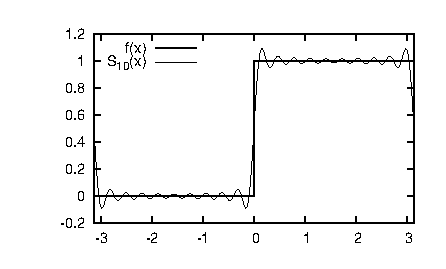
\includegraphics[width=5cm]{obrazky/gibbs_saw10}
            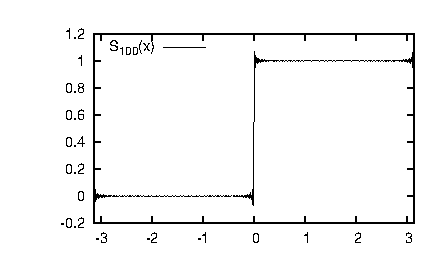
\includegraphics[width=5cm]{obrazky/gibbs_saw100}
        \end{centering}
        \caption{Gibbsov fenomén}
    \end{figure}
\end{frame}

\begin{frame}{Gibbsov fenomén a zvonenie u ideálnych filtrov}
    \tiny
    \begin{figure}
        \subfigure{}{
            
\includegraphics[width=2cm]{obrazky/source_highpass}
        }
        \\
        \subfigure{}{
            
\includegraphics[width=2cm]{obrazky/ideal_highpass_40}
        }
        \subfigure{Frekvencia}{
            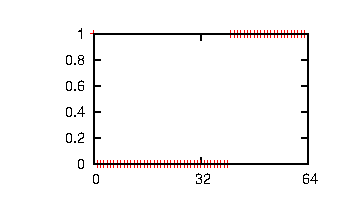
\includegraphics[width=3cm]{obrazky/ideal_highpass_frequency_40}
        }
        \subfigure{Odozva}{
            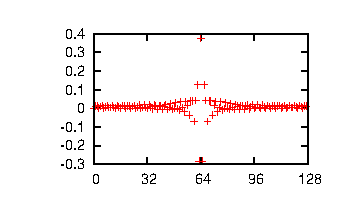
\includegraphics[width=3cm]{obrazky/ideal_highpass_response_40}
        }
        \\
        \subfigure{}{
            
\includegraphics[width=2cm]{obrazky/gauss_highpass_40}
        }
        \subfigure{Frekvencia}{
            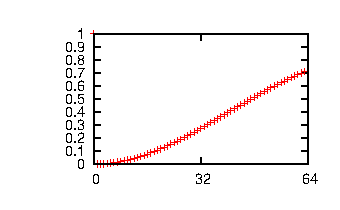
\includegraphics[width=3cm]{obrazky/gauss_highpass_frequency_40}
        }
        \subfigure{Odozva}{
            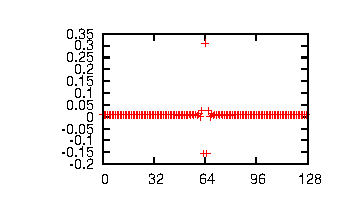
\includegraphics[width=3cm]{obrazky/gauss_highpass_response_40}
        }
    \end{figure}
\end{frame}
%%% }}}

%%% {{{ Faza a magnituda
\subsection{FT - fáza a magnitúda}
\begin{frame}{Súvis medzi fázou a magnitúdou}
    \begin{figure}
        \begin{centering}
        \tiny
        \subfigure{$\phi_1$, mag 1}{
            
\includegraphics[width=2cm]{obrazky/p1m1}
        }
        \subfigure{$\phi_1$, mag 2}{
            
\includegraphics[width=2cm]{obrazky/p1m2}
        }
        \subfigure{$\phi_1$, mag c}{
            
\includegraphics[width=2cm]{obrazky/p1mc}
        }
        \\
        \subfigure{$\phi_2$, mag 1}{
            
\includegraphics[width=2cm]{obrazky/p2m1}
        }
        \subfigure{$\phi_2$, mag 2}{
            
\includegraphics[width=2cm]{obrazky/p2m2}
        }
        \subfigure{$\phi_2$, mag c}{
            
\includegraphics[width=2cm]{obrazky/p2mc}
        }
        \\
        \subfigure{$\phi=0$, mag 1}{
            
\includegraphics[width=2cm]{obrazky/pcm1}
        }
        \subfigure{$\phi=0$, mag 2}{
            
\includegraphics[width=2cm]{obrazky/pcm2}
        }
        \end{centering}
    \end{figure}
\end{frame}
%%% }}}

\def\sipka{\rightarrow}

%%% {{{ Kompresia obrazu a videa
\subsection{Kompresia obrazu a videa}
\begin{frame}{Kompresia obrazu}
    \begin{itemize}
        \item Obraz $\sipka$ transformácia $\sipka$ kvantizácia
          $\sipka$ kompresia
        \item Úlohou transformácie je predpripraviť dáta
        \item FFT vs. DCT
            \begin{itemize}
                \item Komplexné čísla
                \item Dôležitosť fázy FFT
                \item Porovnanie distribúcie energie
            \end{itemize}
    \end{itemize}
\end{frame}
%%% }}}

%%% {{{ FFT vs DCT
\begin{frame}{Porovnanie FFT a DCT}
    \begin{figure}
        \begin{centering}
        \subfigure{Obraz}{
            
\includegraphics[width=3cm]{obrazky/image}
        }
        \\
        \subfigure{FFT}{
            
\includegraphics[width=3cm]{obrazky/dft}
        }
        \subfigure{DCT}{
            
\includegraphics[width=3cm]{obrazky/dct}
        }
        \\
        \subfigure{Histogramy}{
            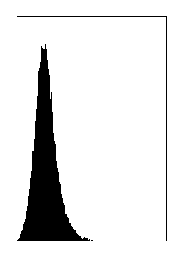
\includegraphics[width=1cm]{obrazky/dft_histogram}
            
\includegraphics[width=1cm]{obrazky/dct_histogram}
            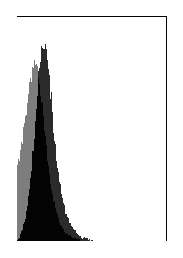
\includegraphics[width=1cm]{obrazky/combined_histogram}
        }
        \end{centering}
    \end{figure}
\end{frame}
%%% }}}

%%% {{{ Kompresia zvuku
\subsection{Kompresia zvuku}
\begin{frame}{Kompresia zvuku}
    \begin{itemize}
        \item Používa sa modifikovaná diskrétna kosínová transformácia
            \item problémy spracovania po úsekoch
            \item riešenie - windowing a modifikovaná transformácia
    \end{itemize}
    \begin{figure}
        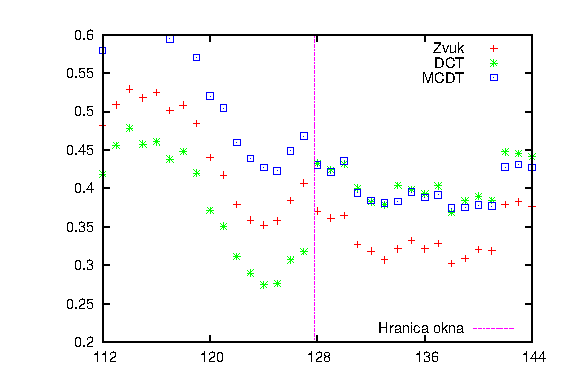
\includegraphics[width=5cm]{obrazky/dct_vs_mdct}
    \end{figure}
\end{frame}
%%% }}}

%%% {{{ Rychle nasobenie polynomov
\subsection{Rýchle násobenie polynómov}
\begin{frame}[Rýchle násobenie polynómov]
    \begin{itemize}
        \item Odvodenie algoritmu na rýchle násobenie polynómov
        \item Súvislosť násobenia polynómov s Fourierovou
        transformáciou
            \begin{itemize}
                \item Všeobecná FT v poli resp. okruhu
                \item Odvodený algoritmus - Radix2 FFT
            \end{itemize}
    \end{itemize}
\end{frame}
%%% }}}


\section{Záver}
%%% {{{ Dalsia praca
\subsection{Ďalšia práca}
\begin{frame}{Ďalšia práca}
    \begin{itemize}
        \item Algoritmy na výpočet rýchlej Fourierovej transformácie
            \begin{itemize}
                \item Radix-2 rýchle algoritmy
                \item Cooley-Tukey pre zložené čísla
                \item Algoritmy pre prvočíselné dĺžky
            \end{itemize}
        \item Použitie v matematike
            \begin{itemize}
                \item Riešenie diferenciálnych rovníc
                \item Ortonormálne systémy
            \end{itemize}
        \item Použitie vo fyzike
            \begin{itemize}
                \item FTIR
                \item NMRI, CT
                \item Kvantová mechanika
            \end{itemize}
    \end{itemize}
\end{frame}
%%% }}}

%%% {{{ Zhrnutie
\begin{frame}{Zhrnutie práce}
    \begin{itemize}
        \item Zozbieranie poznatkov o Fourierovej transformácii
            \begin{itemize}
            \item zjednotenie dôkazov a zosúladenie definícii
            \end{itemize}
        \item Vysvetlenie použitia Fourierovej transformácie v
        informatike
            \begin{itemize}
            \item zamerané na ukážku súvislostí medzi jednotlivými
            aplikáciami a javmi
            \end{itemize}

    \end{itemize}
\end{frame}
%%% }}}

%%% {{{ Koniec
\begin{frame}{Koniec}
    \begin{table}
    \begin{centering}
        \large Ďakujem za pozornosť.
    \end{centering}
    \end{table}
\end{frame}
%%% }}}

\end{document}
